% Created by tikzDevice version 0.12 on 2018-12-10 11:33:33
% !TEX encoding = UTF-8 Unicode
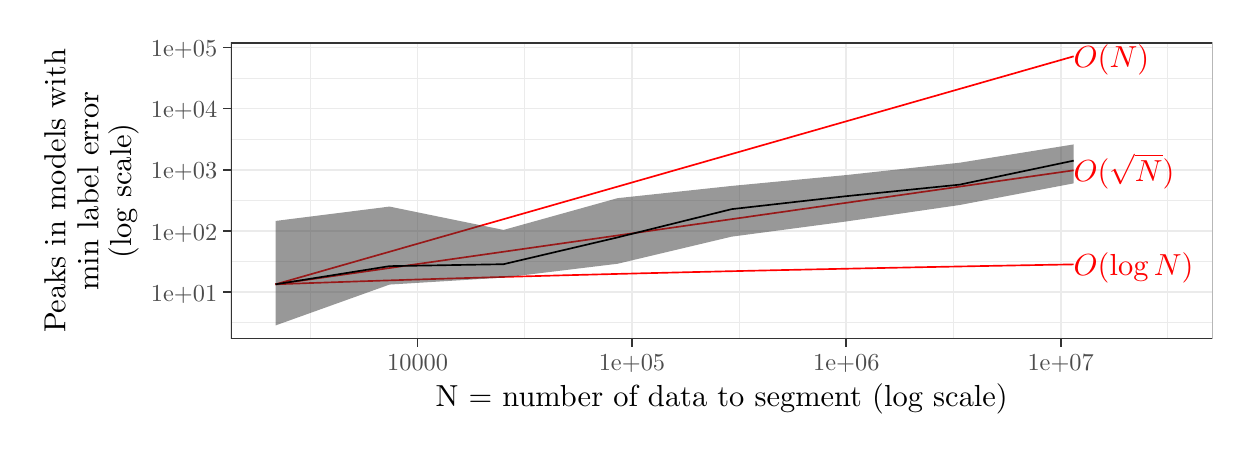
\begin{tikzpicture}[x=1pt,y=1pt]
\definecolor{fillColor}{RGB}{255,255,255}
\path[use as bounding box,fill=fillColor,fill opacity=0.00] (0,0) rectangle (433.62,144.54);
\begin{scope}
\path[clip] (  0.00,  0.00) rectangle (433.62,144.54);
\definecolor{drawColor}{RGB}{255,255,255}
\definecolor{fillColor}{RGB}{255,255,255}

\path[draw=drawColor,line width= 0.6pt,line join=round,line cap=round,fill=fillColor] (  0.00,  0.00) rectangle (433.62,144.54);
\end{scope}
\begin{scope}
\path[clip] ( 73.43, 32.08) rectangle (428.12,139.04);
\definecolor{fillColor}{RGB}{255,255,255}

\path[fill=fillColor] ( 73.43, 32.08) rectangle (428.12,139.04);
\definecolor{drawColor}{gray}{0.92}

\path[draw=drawColor,line width= 0.3pt,line join=round] ( 73.43, 37.86) --
	(428.12, 37.86);

\path[draw=drawColor,line width= 0.3pt,line join=round] ( 73.43, 59.98) --
	(428.12, 59.98);

\path[draw=drawColor,line width= 0.3pt,line join=round] ( 73.43, 82.10) --
	(428.12, 82.10);

\path[draw=drawColor,line width= 0.3pt,line join=round] ( 73.43,104.23) --
	(428.12,104.23);

\path[draw=drawColor,line width= 0.3pt,line join=round] ( 73.43,126.35) --
	(428.12,126.35);

\path[draw=drawColor,line width= 0.3pt,line join=round] (102.18, 32.08) --
	(102.18,139.04);

\path[draw=drawColor,line width= 0.3pt,line join=round] (179.63, 32.08) --
	(179.63,139.04);

\path[draw=drawColor,line width= 0.3pt,line join=round] (257.09, 32.08) --
	(257.09,139.04);

\path[draw=drawColor,line width= 0.3pt,line join=round] (334.54, 32.08) --
	(334.54,139.04);

\path[draw=drawColor,line width= 0.3pt,line join=round] (412.00, 32.08) --
	(412.00,139.04);

\path[draw=drawColor,line width= 0.6pt,line join=round] ( 73.43, 48.92) --
	(428.12, 48.92);

\path[draw=drawColor,line width= 0.6pt,line join=round] ( 73.43, 71.04) --
	(428.12, 71.04);

\path[draw=drawColor,line width= 0.6pt,line join=round] ( 73.43, 93.16) --
	(428.12, 93.16);

\path[draw=drawColor,line width= 0.6pt,line join=round] ( 73.43,115.29) --
	(428.12,115.29);

\path[draw=drawColor,line width= 0.6pt,line join=round] ( 73.43,137.41) --
	(428.12,137.41);

\path[draw=drawColor,line width= 0.6pt,line join=round] (140.90, 32.08) --
	(140.90,139.04);

\path[draw=drawColor,line width= 0.6pt,line join=round] (218.36, 32.08) --
	(218.36,139.04);

\path[draw=drawColor,line width= 0.6pt,line join=round] (295.81, 32.08) --
	(295.81,139.04);

\path[draw=drawColor,line width= 0.6pt,line join=round] (373.27, 32.08) --
	(373.27,139.04);
\definecolor{drawColor}{RGB}{255,0,0}

\path[draw=drawColor,line width= 0.6pt,line join=round] ( 89.56, 51.80) --
	( 92.47, 51.91) --
	( 95.38, 52.02) --
	( 98.30, 52.12) --
	(101.21, 52.23) --
	(104.12, 52.33) --
	(107.04, 52.43) --
	(109.95, 52.53) --
	(112.86, 52.63) --
	(115.78, 52.73) --
	(118.69, 52.83) --
	(121.60, 52.93) --
	(124.52, 53.02) --
	(127.43, 53.12) --
	(130.34, 53.21) --
	(133.26, 53.30) --
	(136.17, 53.40) --
	(139.08, 53.49) --
	(142.00, 53.58) --
	(144.91, 53.67) --
	(147.82, 53.76) --
	(150.74, 53.85) --
	(153.65, 53.93) --
	(156.56, 54.02) --
	(159.48, 54.10) --
	(162.39, 54.19) --
	(165.30, 54.27) --
	(168.21, 54.36) --
	(171.13, 54.44) --
	(174.04, 54.52) --
	(176.95, 54.60) --
	(179.87, 54.68) --
	(182.78, 54.76) --
	(185.69, 54.84) --
	(188.61, 54.92) --
	(191.52, 55.00) --
	(194.43, 55.08) --
	(197.35, 55.15) --
	(200.26, 55.23) --
	(203.17, 55.30) --
	(206.09, 55.38) --
	(209.00, 55.45) --
	(211.91, 55.53) --
	(214.83, 55.60) --
	(217.74, 55.67) --
	(220.65, 55.75) --
	(223.57, 55.82) --
	(226.48, 55.89) --
	(229.39, 55.96) --
	(232.31, 56.03) --
	(235.22, 56.10) --
	(238.13, 56.17) --
	(241.05, 56.24) --
	(243.96, 56.30) --
	(246.87, 56.37) --
	(249.79, 56.44) --
	(252.70, 56.51) --
	(255.61, 56.57) --
	(258.53, 56.64) --
	(261.44, 56.70) --
	(264.35, 56.77) --
	(267.27, 56.83) --
	(270.18, 56.90) --
	(273.09, 56.96) --
	(276.01, 57.02) --
	(278.92, 57.08) --
	(281.83, 57.15) --
	(284.75, 57.21) --
	(287.66, 57.27) --
	(290.57, 57.33) --
	(293.49, 57.39) --
	(296.40, 57.45) --
	(299.31, 57.51) --
	(302.23, 57.57) --
	(305.14, 57.63) --
	(308.05, 57.69) --
	(310.97, 57.75) --
	(313.88, 57.81) --
	(316.79, 57.86) --
	(319.71, 57.92) --
	(322.62, 57.98) --
	(325.53, 58.04) --
	(328.45, 58.09) --
	(331.36, 58.15) --
	(334.27, 58.20) --
	(337.19, 58.26) --
	(340.10, 58.31) --
	(343.01, 58.37) --
	(345.93, 58.42) --
	(348.84, 58.48) --
	(351.75, 58.53) --
	(354.67, 58.59) --
	(357.58, 58.64) --
	(360.49, 58.69) --
	(363.41, 58.74) --
	(366.32, 58.80) --
	(369.23, 58.85) --
	(372.14, 58.90) --
	(375.06, 58.95) --
	(377.97, 59.00);

\path[draw=drawColor,line width= 0.6pt,line join=round] ( 89.56, 51.80) --
	( 92.47, 52.22) --
	( 95.38, 52.64) --
	( 98.30, 53.05) --
	(101.21, 53.47) --
	(104.12, 53.88) --
	(107.04, 54.30) --
	(109.95, 54.72) --
	(112.86, 55.13) --
	(115.78, 55.55) --
	(118.69, 55.96) --
	(121.60, 56.38) --
	(124.52, 56.80) --
	(127.43, 57.21) --
	(130.34, 57.63) --
	(133.26, 58.04) --
	(136.17, 58.46) --
	(139.08, 58.88) --
	(142.00, 59.29) --
	(144.91, 59.71) --
	(147.82, 60.12) --
	(150.74, 60.54) --
	(153.65, 60.96) --
	(156.56, 61.37) --
	(159.48, 61.79) --
	(162.39, 62.20) --
	(165.30, 62.62) --
	(168.21, 63.04) --
	(171.13, 63.45) --
	(174.04, 63.87) --
	(176.95, 64.28) --
	(179.87, 64.70) --
	(182.78, 65.12) --
	(185.69, 65.53) --
	(188.61, 65.95) --
	(191.52, 66.37) --
	(194.43, 66.78) --
	(197.35, 67.20) --
	(200.26, 67.61) --
	(203.17, 68.03) --
	(206.09, 68.45) --
	(209.00, 68.86) --
	(211.91, 69.28) --
	(214.83, 69.69) --
	(217.74, 70.11) --
	(220.65, 70.53) --
	(223.57, 70.94) --
	(226.48, 71.36) --
	(229.39, 71.77) --
	(232.31, 72.19) --
	(235.22, 72.61) --
	(238.13, 73.02) --
	(241.05, 73.44) --
	(243.96, 73.85) --
	(246.87, 74.27) --
	(249.79, 74.69) --
	(252.70, 75.10) --
	(255.61, 75.52) --
	(258.53, 75.93) --
	(261.44, 76.35) --
	(264.35, 76.77) --
	(267.27, 77.18) --
	(270.18, 77.60) --
	(273.09, 78.01) --
	(276.01, 78.43) --
	(278.92, 78.85) --
	(281.83, 79.26) --
	(284.75, 79.68) --
	(287.66, 80.09) --
	(290.57, 80.51) --
	(293.49, 80.93) --
	(296.40, 81.34) --
	(299.31, 81.76) --
	(302.23, 82.17) --
	(305.14, 82.59) --
	(308.05, 83.01) --
	(310.97, 83.42) --
	(313.88, 83.84) --
	(316.79, 84.25) --
	(319.71, 84.67) --
	(322.62, 85.09) --
	(325.53, 85.50) --
	(328.45, 85.92) --
	(331.36, 86.33) --
	(334.27, 86.75) --
	(337.19, 87.17) --
	(340.10, 87.58) --
	(343.01, 88.00) --
	(345.93, 88.41) --
	(348.84, 88.83) --
	(351.75, 89.25) --
	(354.67, 89.66) --
	(357.58, 90.08) --
	(360.49, 90.49) --
	(363.41, 90.91) --
	(366.32, 91.33) --
	(369.23, 91.74) --
	(372.14, 92.16) --
	(375.06, 92.58) --
	(377.97, 92.99);

\path[draw=drawColor,line width= 0.6pt,line join=round] ( 89.56, 51.80) --
	( 92.47, 52.64) --
	( 95.38, 53.47) --
	( 98.30, 54.30) --
	(101.21, 55.13) --
	(104.12, 55.96) --
	(107.04, 56.80) --
	(109.95, 57.63) --
	(112.86, 58.46) --
	(115.78, 59.29) --
	(118.69, 60.12) --
	(121.60, 60.96) --
	(124.52, 61.79) --
	(127.43, 62.62) --
	(130.34, 63.45) --
	(133.26, 64.28) --
	(136.17, 65.12) --
	(139.08, 65.95) --
	(142.00, 66.78) --
	(144.91, 67.61) --
	(147.82, 68.45) --
	(150.74, 69.28) --
	(153.65, 70.11) --
	(156.56, 70.94) --
	(159.48, 71.77) --
	(162.39, 72.61) --
	(165.30, 73.44) --
	(168.21, 74.27) --
	(171.13, 75.10) --
	(174.04, 75.93) --
	(176.95, 76.77) --
	(179.87, 77.60) --
	(182.78, 78.43) --
	(185.69, 79.26) --
	(188.61, 80.09) --
	(191.52, 80.93) --
	(194.43, 81.76) --
	(197.35, 82.59) --
	(200.26, 83.42) --
	(203.17, 84.25) --
	(206.09, 85.09) --
	(209.00, 85.92) --
	(211.91, 86.75) --
	(214.83, 87.58) --
	(217.74, 88.41) --
	(220.65, 89.25) --
	(223.57, 90.08) --
	(226.48, 90.91) --
	(229.39, 91.74) --
	(232.31, 92.58) --
	(235.22, 93.41) --
	(238.13, 94.24) --
	(241.05, 95.07) --
	(243.96, 95.90) --
	(246.87, 96.74) --
	(249.79, 97.57) --
	(252.70, 98.40) --
	(255.61, 99.23) --
	(258.53,100.06) --
	(261.44,100.90) --
	(264.35,101.73) --
	(267.27,102.56) --
	(270.18,103.39) --
	(273.09,104.22) --
	(276.01,105.06) --
	(278.92,105.89) --
	(281.83,106.72) --
	(284.75,107.55) --
	(287.66,108.38) --
	(290.57,109.22) --
	(293.49,110.05) --
	(296.40,110.88) --
	(299.31,111.71) --
	(302.23,112.54) --
	(305.14,113.38) --
	(308.05,114.21) --
	(310.97,115.04) --
	(313.88,115.87) --
	(316.79,116.70) --
	(319.71,117.54) --
	(322.62,118.37) --
	(325.53,119.20) --
	(328.45,120.03) --
	(331.36,120.87) --
	(334.27,121.70) --
	(337.19,122.53) --
	(340.10,123.36) --
	(343.01,124.19) --
	(345.93,125.03) --
	(348.84,125.86) --
	(351.75,126.69) --
	(354.67,127.52) --
	(357.58,128.35) --
	(360.49,129.19) --
	(363.41,130.02) --
	(366.32,130.85) --
	(369.23,131.68) --
	(372.14,132.51) --
	(375.06,133.35) --
	(377.97,134.18);

\node[text=drawColor,anchor=base west,inner sep=0pt, outer sep=0pt, scale=  1.10] at (377.97,130.10) {$O(N)$};

\node[text=drawColor,anchor=base west,inner sep=0pt, outer sep=0pt, scale=  1.10] at (377.97, 54.92) {$O(\log N)$};

\node[text=drawColor,anchor=base west,inner sep=0pt, outer sep=0pt, scale=  1.10] at (377.97, 88.91) {$O(\sqrt N)$};
\definecolor{fillColor}{RGB}{51,51,51}

\path[fill=fillColor,fill opacity=0.50] ( 89.56, 74.70) --
	(130.76, 79.89) --
	(171.96, 71.45) --
	(213.16, 82.93) --
	(254.36, 87.35) --
	(295.57, 91.26) --
	(336.77, 95.74) --
	(377.97,102.35) --
	(377.97, 88.28) --
	(336.77, 80.46) --
	(295.57, 74.48) --
	(254.36, 69.02) --
	(213.16, 59.23) --
	(171.96, 54.23) --
	(130.76, 51.71) --
	( 89.56, 36.94) --
	cycle;
\definecolor{drawColor}{RGB}{0,0,0}

\path[draw=drawColor,line width= 0.6pt,line join=round] ( 89.56, 51.80) --
	(130.76, 58.37) --
	(171.96, 59.07) --
	(213.16, 68.75) --
	(254.36, 78.96) --
	(295.57, 83.63) --
	(336.77, 87.82) --
	(377.97, 96.49);
\definecolor{drawColor}{gray}{0.20}

\path[draw=drawColor,line width= 0.6pt,line join=round,line cap=round] ( 73.43, 32.08) rectangle (428.12,139.04);
\end{scope}
\begin{scope}
\path[clip] (  0.00,  0.00) rectangle (433.62,144.54);
\definecolor{drawColor}{gray}{0.30}

\node[text=drawColor,anchor=base east,inner sep=0pt, outer sep=0pt, scale=  0.88] at ( 68.48, 45.67) {1e+01};

\node[text=drawColor,anchor=base east,inner sep=0pt, outer sep=0pt, scale=  0.88] at ( 68.48, 67.79) {1e+02};

\node[text=drawColor,anchor=base east,inner sep=0pt, outer sep=0pt, scale=  0.88] at ( 68.48, 89.91) {1e+03};

\node[text=drawColor,anchor=base east,inner sep=0pt, outer sep=0pt, scale=  0.88] at ( 68.48,112.03) {1e+04};

\node[text=drawColor,anchor=base east,inner sep=0pt, outer sep=0pt, scale=  0.88] at ( 68.48,134.16) {1e+05};
\end{scope}
\begin{scope}
\path[clip] (  0.00,  0.00) rectangle (433.62,144.54);
\definecolor{drawColor}{gray}{0.20}

\path[draw=drawColor,line width= 0.6pt,line join=round] ( 70.68, 48.92) --
	( 73.43, 48.92);

\path[draw=drawColor,line width= 0.6pt,line join=round] ( 70.68, 71.04) --
	( 73.43, 71.04);

\path[draw=drawColor,line width= 0.6pt,line join=round] ( 70.68, 93.16) --
	( 73.43, 93.16);

\path[draw=drawColor,line width= 0.6pt,line join=round] ( 70.68,115.29) --
	( 73.43,115.29);

\path[draw=drawColor,line width= 0.6pt,line join=round] ( 70.68,137.41) --
	( 73.43,137.41);
\end{scope}
\begin{scope}
\path[clip] (  0.00,  0.00) rectangle (433.62,144.54);
\definecolor{drawColor}{gray}{0.20}

\path[draw=drawColor,line width= 0.6pt,line join=round] (140.90, 29.33) --
	(140.90, 32.08);

\path[draw=drawColor,line width= 0.6pt,line join=round] (218.36, 29.33) --
	(218.36, 32.08);

\path[draw=drawColor,line width= 0.6pt,line join=round] (295.81, 29.33) --
	(295.81, 32.08);

\path[draw=drawColor,line width= 0.6pt,line join=round] (373.27, 29.33) --
	(373.27, 32.08);
\end{scope}
\begin{scope}
\path[clip] (  0.00,  0.00) rectangle (433.62,144.54);
\definecolor{drawColor}{gray}{0.30}

\node[text=drawColor,anchor=base,inner sep=0pt, outer sep=0pt, scale=  0.88] at (140.90, 20.63) {10000};

\node[text=drawColor,anchor=base,inner sep=0pt, outer sep=0pt, scale=  0.88] at (218.36, 20.63) {1e+05};

\node[text=drawColor,anchor=base,inner sep=0pt, outer sep=0pt, scale=  0.88] at (295.81, 20.63) {1e+06};

\node[text=drawColor,anchor=base,inner sep=0pt, outer sep=0pt, scale=  0.88] at (373.27, 20.63) {1e+07};
\end{scope}
\begin{scope}
\path[clip] (  0.00,  0.00) rectangle (433.62,144.54);
\definecolor{drawColor}{RGB}{0,0,0}

\node[text=drawColor,anchor=base,inner sep=0pt, outer sep=0pt, scale=  1.10] at (250.78,  7.62) {N = number of data to segment (log scale)};
\end{scope}
\begin{scope}
\path[clip] (  0.00,  0.00) rectangle (433.62,144.54);
\definecolor{drawColor}{RGB}{0,0,0}

\node[text=drawColor,rotate= 90.00,anchor=base,inner sep=0pt, outer sep=0pt, scale=  1.10] at ( 13.63, 85.56) {Peaks in models with};

\node[text=drawColor,rotate= 90.00,anchor=base,inner sep=0pt, outer sep=0pt, scale=  1.10] at ( 25.51, 85.56) {min label error};

\node[text=drawColor,rotate= 90.00,anchor=base,inner sep=0pt, outer sep=0pt, scale=  1.10] at ( 37.39, 85.56) {(log scale)};
\end{scope}
\end{tikzpicture}
